\documentclass[notes,11pt, aspectratio=169, xcolor=table]{beamer}

\usepackage{pgfpages}
% These slides also contain speaker notes. You can print just the slides,
% just the notes, or both, depending on the setting below. Comment out the want
% you want.
\setbeameroption{hide notes} % Only slide
%\setbeameroption{show only notes} % Only notes
%\setbeameroption{show notes on second screen=right} % Both


\newtheorem{proposition}{Proposition}
\newcommand{\blue}[1]{\textcolor{blue}{#1}}
\newcommand{\white}[1]{\textcolor{white}{#1}}

\usepackage{helvet}
\usepackage[default]{lato}
\usepackage{array}
\usepackage{tikz}
\usetikzlibrary{shapes.geometric}
\usepackage{pgfplots}
\usetikzlibrary{patterns, pgfplots.fillbetween}
\usepackage{graphicx}
\usepackage{verbatim}
\setbeamertemplate{note page}{\pagecolor{yellow!5}\insertnote}
\usetikzlibrary{positioning}
\usetikzlibrary{snakes}
\usetikzlibrary{calc}
\usetikzlibrary{arrows}
\usetikzlibrary{decorations.markings}
\usetikzlibrary{shapes.misc}
\usetikzlibrary{matrix,shapes,arrows,fit,tikzmark}
\usepackage{amsmath}
\usepackage{mathpazo}
\usepackage{hyperref}
\usepackage{lipsum}
\usepackage{multimedia}
\usepackage{graphicx}
\usepackage{multirow}
\usepackage{graphicx}
\usepackage{dcolumn}
\usepackage{bbm}
\usepackage{emoji}
\usepackage[style=authoryear,sorting=nyt,uniquename=false]{biblatex}

\addbibresource{references.bib} 

\newcolumntype{d}[0]{D{.}{.}{5}}

\def\@@mybluebox[#1][#2]#3{
    \sbox\mytempbox{#3}%
    \mytemplen\ht\mytempbox
    \advance\mytemplen #1\relax
    \ht\mytempbox\mytemplen
    \mytemplen\dp\mytempbox
    \advance\mytemplen #2\relax
    \dp\mytempbox\mytemplen
    \colorbox{myblue}{\hspace{1em}\usebox{\mytempbox}\hspace{1em}}}


\usepackage{changepage}
\usepackage{appendixnumberbeamer}
\newcommand{\beginbackup}{
   \newcounter{framenumbervorappendix}
   \setcounter{framenumbervorappendix}{\value{framenumber}}
   \setbeamertemplate{footline}
   {
     \leavevmode%
     \hline
     box{%
       \begin{beamercolorbox}[wd=\paperwidth,ht=2.25ex,dp=1ex,right]{footlinecolor}%
%         \insertframenumber  \hspace*{2ex} 
       \end{beamercolorbox}}%
     \vskip0pt%
   }
 }
\newcommand{\backupend}{
   \addtocounter{framenumbervorappendix}{-\value{framenumber}}
   \addtocounter{framenumber}{\value{framenumbervorappendix}} 
}


\usepackage{graphicx}
\usepackage[space]{grffile}
\usepackage{booktabs}

% These are my colors -- there are many like them, but these ones are mine.
\definecolor{blue}{RGB}{0,114,178}
\definecolor{red}{RGB}{213,94,0}
\definecolor{yellow}{RGB}{240,228,66}
\definecolor{green}{RGB}{0,158,115}

\hypersetup{
  colorlinks=false,
  linkbordercolor = {white},
  linkcolor = {blue}
}


%% I use a beige off white for my background
\definecolor{MyBackground}{RGB}{255,253,218}

%% Uncomment this if you want to change the background color to something else
%\setbeamercolor{background canvas}{bg=MyBackground}

%% Change the bg color to adjust your transition slide background color!
\newenvironment{transitionframe}{
  \setbeamercolor{background canvas}{bg=yellow}
  \begin{frame}}{
    \end{frame}
}

\setbeamercolor{frametitle}{fg=blue}
\setbeamercolor{title}{fg=blue}
\setbeamertemplate{footline}[frame number]
\setbeamertemplate{navigation symbols}{} 
\setbeamertemplate{itemize items}{-}
\setbeamercolor{itemize item}{fg=blue}
\setbeamercolor{itemize subitem}{fg=blue}
\setbeamercolor{enumerate item}{fg=blue}
\setbeamercolor{enumerate subitem}{fg=blue}
\setbeamercolor{button}{bg=MyBackground,fg=blue,}



% If you like road maps, rather than having clutter at the top, have a roadmap show up at the end of each section 
% (and after your introduction)
% Uncomment this is if you want the roadmap!
% \AtBeginSection[]
% {
%    \begin{frame}
%        \frametitle{Roadmap of Talk}
%        \tableofcontents[currentsection]
%    \end{frame}
% }
\setbeamercolor{section in toc}{fg=blue}
\setbeamercolor{subsection in toc}{fg=red}
\setbeamersize{text margin left=1em,text margin right=1em} 

\newenvironment{wideitemize}{\itemize\addtolength{\itemsep}{10pt}}{\enditemize}

\usepackage{environ}
\NewEnviron{videoframe}[1]{
  \begin{frame}
    \vspace{-8pt}
    \begin{columns}[onlytextwidth, T] % align columns
      \begin{column}{.58\textwidth}
        \begin{minipage}[t][\textheight][t]
          {\dimexpr\textwidth}
          \vspace{8pt}
          \hspace{4pt} {\Large \sc \textcolor{blue}{#1}}
          \vspace{8pt}
          
          \BODY
        \end{minipage}
      \end{column}%
      \hfill%
      \begin{column}{.42\textwidth}
        \colorbox{green!20}{\begin{minipage}[t][1.2\textheight][t]
            {\dimexpr\textwidth}
            Face goes here
          \end{minipage}}
      \end{column}%
    \end{columns}
  \end{frame}
}

\title[]{International Trade: Lecture 7}
\subtitle[]{Production in the Short and the Long Run}
\author[Góes]
{Carlos Góes\inst{1}}
\date{Fall 2025}
\institute[GWU]{\inst{1} George Washington University }



\begin{document}

%%% TIKZ STUFF
\tikzset{   
        every picture/.style={remember picture,baseline},
        every node/.style={anchor=base,align=center,outer sep=1.5pt},
        every path/.style={thick},
        }
\newcommand\marktopleft[1]{%
    \tikz[overlay,remember picture] 
        \node (marker-#1-a) at (-.3em,.3em) {};%
}
\newcommand\markbottomright[2]{%
    \tikz[overlay,remember picture] 
        \node (marker-#1-b) at (0em,0em) {};%
}
\tikzstyle{every picture}+=[remember picture] 
\tikzstyle{mybox} =[draw=black, very thick, rectangle, inner sep=10pt, inner ysep=20pt]
\tikzstyle{fancytitle} =[draw=black,fill=red, text=white]
%%%% END TIKZ STUFF



%----------------------------------------------------------------------%
%-------------------       TITLE PAGE       ---------------------------%
%----------------------------------------------------------------------%





%----------------------------------------------------------------------%






%----------------------------------------------------------------------%
%----------------------------------------------------------------------%

%----------------------------------------------------------------------%
\frame{\titlepage}
\addtocounter{framenumber}{-1}
%----------------------------------------------------------------------%



%----------------------------------------------------------------------%
%----------------------------------------------------------------------%

\section{Intro and recap}

\begin{frame}{Recap}
\blue{What have we seen so far?}
\begin{wideitemize}
    \item<2-> Trade can lead to welfare gains. \blue{How?}
    \item<3-> Change in relative prices $\rightarrow$ specialization $\rightarrow$ expansion of consumption choices
    \item<3-> Both countries can gain from trade openness
\end{wideitemize}

\onslide<4->{
\vspace{12pt}
\blue{But what assumptions have driven those results?}
\begin{wideitemize}
    \item<5-> Only one factor of production: labor
    \item<6-> Labor is mobile across sectors
    \item<7-> Economy can always adjust proportionately, workers gain (real income $\uparrow$) 
\end{wideitemize}
}

\end{frame}

\begin{frame}{Limits}


\begin{columns}[T] % align columns
\begin{column}{.4\textwidth}
\centering
\onslide<3->{
  \makebox[\linewidth][c]{
    \resizebox{\linewidth}{!}{
    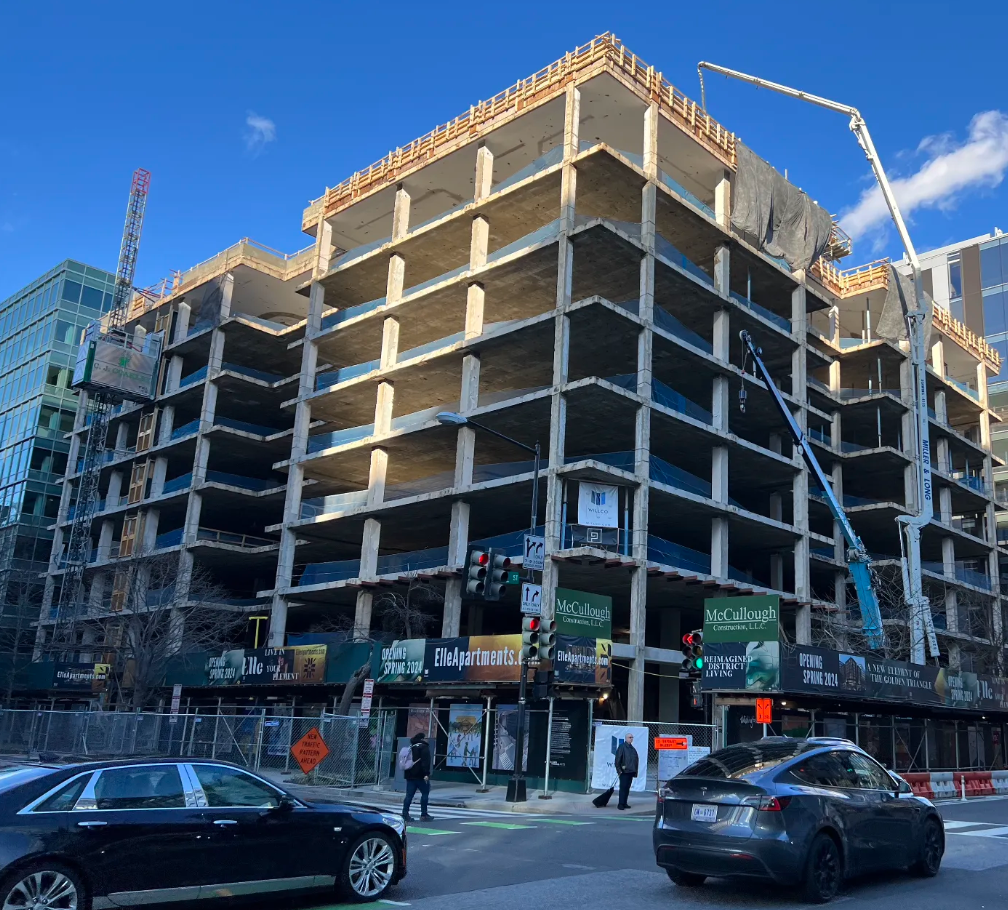
\includegraphics[width=\linewidth]{figs/peacecrops.png} 
      }
    }
    \\
    \vspace{12pt}
    { \scriptsize PeaceCorps HQ converted into apt building \\ 1111 20th ST NW}
}
\end{column}%
\hfill%
\begin{column}{.6\textwidth}
\blue{What about those assumptions?}

\begin{wideitemize}
    \item<1-> Production often use \blue{more than one factor}
    \begin{itemize}
        \item this class uses labor (me) + capital (computer, projector) + structures (building)
    \end{itemize}
    
    \item<2-> Factors \blue{cannot always freely adjust} 
    \begin{itemize}
        \item e.g.: can an office building become an apartment building?
        \item<3-> yes, but costly, lengthy 
    \end{itemize}

    
    \item<4-> What happens if we \blue{relax those assumptions}?
    \begin{itemize}
        \item some factor owners can be worse off from trade over short run
        \item Ricardian logic can be though off as long run
    \end{itemize}

    
\end{wideitemize}
\end{column}%
\end{columns}

\end{frame}



\begin{frame}{Example: China trade shock}


\begin{columns}[T] % align columns
\begin{column}{.45\textwidth}
\onslide<2->{
\centering
  \makebox[\linewidth][c]{
    \resizebox{\linewidth}{!}{
    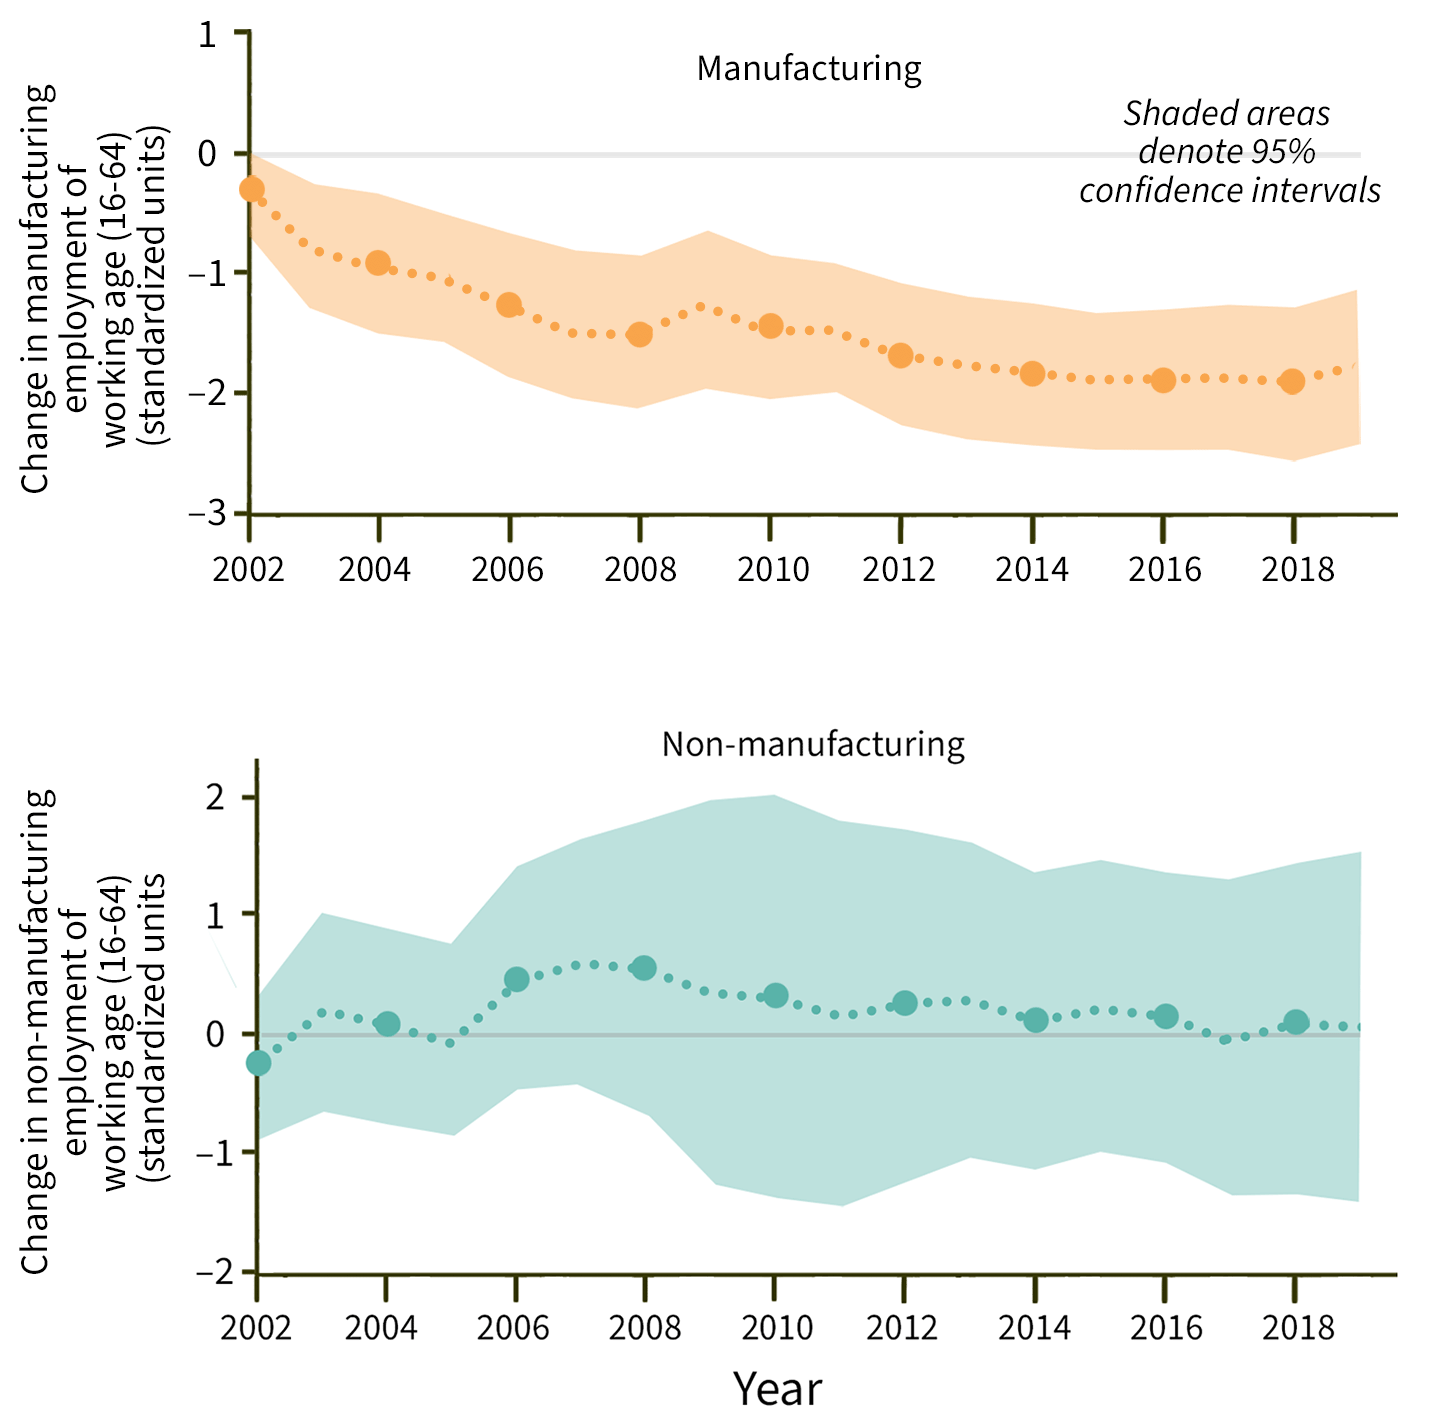
\includegraphics[width=\linewidth]{figs/shock_fig_1a-b_3.png} 
      }
    }
    \vspace{12pt}
    { \scriptsize
    Source: \href{https://www.nber.org/system/files/working_papers/w29401/w29401.pdf}{Autor, Dorn \& Hanson (2021)}
    }
}
\end{column}%
\hfill%
\begin{column}{.55\textwidth}
{\small
\begin{wideitemize}
    \item<1-> China's share in world manufacturing exports rose from 3.1\% in 1991 to 17.6\% in 2015

    \item<2-> US regions more exposed to Chinese import competition saw (relative) losses in manufacturing employment growth

    \item<3-> Effects persist many years into the future, due to frictions for labor mobility

    \item<4-> Prices did fall about 1.5\%: about ~95\% of US population saw real income growth due to shock; 5\% losses 

    
\end{wideitemize}
}
\end{column}%
\end{columns}

\end{frame}



\section{Production Function}

\begin{frame}{}
\addtocounter{framenumber}{-1}

\Huge \blue{The Production Function}
\end{frame}



\begin{frame}{Gelato Factory}

\begin{columns}[T] % align columns
\begin{column}{.4\textwidth}
  \makebox[\linewidth][c]{
    \resizebox{\linewidth}{!}{
    
\includegraphics[width=\linewidth]{figs/dolcezza-mascarpone-and-fig-contrast-edit.png}
      }
    }
\end{column}%
\hfill%
\begin{column}{.6\textwidth}
  \begin{wideitemize}
    \item Example: Gelato Factory
    \item Inputs:
    \begin{itemize}
        \item Milk, Sugar, Salt
        \item Chocolate/Strawberry
        \item Cones/cups/containers
        \item Labor (scoopers + cashier)
    \end{itemize}
    \item Capital:
    \begin{itemize}
        \item Freezer, Machines 
        \item Refrigerated trucks
        \item Factory/building
    \end{itemize}
    \item Intangibles:
    \begin{itemize}
        \item License
        \item Recipe
        \item Business environment, Property rights
    \end{itemize}
    
  \end{wideitemize}
\end{column}%
\end{columns}

\end{frame}


\begin{frame}{The Production Function}

\begin{wideitemize}
\item we are interested in modeling the production of value added
t
\item “factor‐based” representation of the production function:

\begin{equation*}
\underbrace{Y}_{\substack{\text{output}\\\text{value added}}} = F(\underbrace{A}_{\substack{\text{technology}\\\text{institutions}\\\text{ideas}}}, \underbrace{K}_{\text{capital}} , \underbrace{L}_{\text{labor}})
\end{equation*}

\item $F(A, K, L)$ is your production function. If $F(\cdot, \cdot, \cdot)$ is Cobb-Douglas, then:

\begin{equation*}
    Y = A \cdot K^{\beta} L^{1-\beta}, \qquad 0 \le \beta \le 1  
\end{equation*}

\end{wideitemize}

\end{frame}

\begin{frame}{The Production Function}
  \huge{Marginal Product: extra output produced by increasing one factor while keeping all the other factors fixed.} \\
  \vspace{20pt}
  \Large{recall: economic agents make decision by ``reasoning at the margin’’}
\end{frame}

\begin{frame}{Production Function}
  \Large{\textcolor{blue}{Diminishing Marginal Product}: Extra output produced by increasing one factor
while keeping all the other fixed is decreasing in the one increasing factor.} \\
  \vspace{20pt}
  \normalsize With Cobb-Douglas Technology, the Marginal Product of Labor and Capital are:
  \vspace{20pt}
  \begin{columns}[T] % align columns
\begin{column}{.5\textwidth}
\begin{equation*}
  MPL \equiv \frac{\partial Y}{\partial L} = \underbrace{(1-\beta) \bar{Z} \left( \frac{K}{L} \right)^{\beta}}_{\text{decreasing in } L}
\end{equation*}
\end{column}%
\hfill%
\begin{column}{.5\textwidth}
\begin{equation*}
  MPK \equiv \frac{\partial Y}{\partial K} = \underbrace{\beta \bar{Z} \left( \frac{L}{K} \right)^{1-\beta}}_{\text{decreasing in } K}
\end{equation*}

\end{column}%
\end{columns}
\end{frame}


\begin{frame}{Example: Labor}

\begin{columns}[T] % align columns
\begin{column}{.6\textwidth}
  \makebox[\linewidth][c]{
    \resizebox{\linewidth}{!}{

    \begin{tikzpicture}
    \pgfmathsetmacro{\alpha}{1/3}    % preference for computers
    \pgfmathsetmacro{\K}{1}    % labor endowment
    \pgfmathsetmacro{\A}{1}    % labor endowment
    
    \centering
    \begin{axis}[
        ylabel={$Y = A \times K^{1/3} L^{2/3}$ },
        xlabel={Used labor input: $L$},
        ymin=0, ymax=5,
        xmin=0, xmax=5,
        yticklabel=\empty,
        xticklabel=\empty,
        axis lines=left,
        enlargelimits=false,
        clip=false,
        axis on top,
        scaled x ticks=false,
        width=9cm, height=7cm,
        title style={font=\bfseries}
    ]
    
    % PPF: Q_C = (L/a_C) - (a_R/a_C) * Q_R
    \addplot[thick, red, domain=0:4] {\A*\K^(\alpha)*x^(1-\alpha)};
    
    \addplot[dashed, gray] coordinates {(0,{\A*\K^(\alpha)*1^(1-\alpha)}) (1,{\A*\K^(\alpha)*1^(1-\alpha)})};
    \addplot[dashed, gray] coordinates {(1,{\A*\K^(\alpha)*1^(1-\alpha)}) ({\A*\K^(\alpha)*1^(1-\alpha)},0) };
    \addplot[mark=*, only marks, black, mark size=1pt] coordinates {(1, {\A*\K^(\alpha)*1^(1-\alpha)} )};
    
    \addplot[dashed, gray] coordinates {(0,{\A*\K^(\alpha)*2^(1-\alpha)}) (2,{\A*\K^(\alpha)*2^(1-\alpha)})};
    \addplot[dashed, gray] coordinates {(2,{\A*\K^(\alpha)*2^(1-\alpha)}) (2,0)};
    
    \addplot[mark=*, only marks, black, mark size=1pt] coordinates {(2, {\A*\K^(\alpha)*2^(1-\alpha)} )};
    
    \addplot[dashed, gray] coordinates {(0,{\A*\K^(\alpha)*3^(1-\alpha)}) (3,{\A*\K^(\alpha)*3^(1-\alpha)})};
    \addplot[dashed, gray] coordinates {(3,{\A*\K^(\alpha)*3^(1-\alpha)}) (3,0)};
    \addplot[mark=*, only marks, black, mark size=1pt] coordinates {(3, {\A*\K^(\alpha)*3^(1-\alpha)} )};
    
    \addplot[dashed, gray] coordinates {(0,{\A*\K^(\alpha)*4^(1-\alpha)}) (4,{\A*\K^(\alpha)*4^(1-\alpha)})};
    \addplot[dashed, gray] coordinates {(4,{\A*\K^(\alpha)*4^(1-\alpha)}) (4,0)};
    \addplot[mark=*, only marks, black, mark size=1pt] coordinates {(4, {\A*\K^(\alpha)*4^(1-\alpha)} )};
    
    \end{axis}
    
    \end{tikzpicture}
    
      }
    }
\end{column}%
\hfill%
\begin{column}{.4\textwidth}
\begin{equation*}
    Y = \bar{Z} K^{1/3} L^{2/3}
\end{equation*}
\begin{table}[]
\begin{tabular}{
>{\columncolor[HTML]{E6B9B8}}l 
>{\columncolor[HTML]{E6B9B8}}r }
\multicolumn{2}{c}{\cellcolor[HTML]{FFFFFF}$L$ and $Y$ when $K=1$ and $\bar{Z}=1$} \\
\cellcolor[HTML]{953735} \textbf{L}                      & \cellcolor[HTML]{953735} \textbf{Y}                    \\
1                     & 1                    \\
2                     & 1.59                    \\
3                        & 2.08                     \\
4                        & 2.52                    
\end{tabular}
\end{table}
\end{column}%
\end{columns}

\end{frame}

\begin{frame}{Example: Capital}

\begin{columns}[T] % align columns
\begin{column}{.6\textwidth}
  \makebox[\linewidth][c]{
    \resizebox{\linewidth}{!}{
  
    \begin{tikzpicture}
    \pgfmathsetmacro{\alpha}{2/3}    % preference for computers
    \pgfmathsetmacro{\K}{1}    % labor endowment
    \pgfmathsetmacro{\A}{1}    % labor endowment
    
    \centering
    \begin{axis}[
        ylabel={$Y = A \times K^{1/3} L^{2/3}$ },
        xlabel={Used capital input: $K$},
        ymin=0, ymax=5,
        xmin=0, xmax=5,
        yticklabel=\empty,
        xticklabel=\empty,
        axis lines=left,
        enlargelimits=false,
        clip=false,
        axis on top,
        scaled x ticks=false,
        width=9cm, height=7cm,
        title style={font=\bfseries}
    ]
    
    % PPF: Q_C = (L/a_C) - (a_R/a_C) * Q_R
    \addplot[thick, red, domain=0:4] {\A*\K^(\alpha)*x^(1-\alpha)};
    
    \addplot[dashed, gray] coordinates {(0,{\A*\K^(\alpha)*1^(1-\alpha)}) (1,{\A*\K^(\alpha)*1^(1-\alpha)})};
    \addplot[dashed, gray] coordinates {(1,{\A*\K^(\alpha)*1^(1-\alpha)}) ({\A*\K^(\alpha)*1^(1-\alpha)},0) };
    \addplot[mark=*, only marks, black, mark size=1pt] coordinates {(1, {\A*\K^(\alpha)*1^(1-\alpha)} )};
    
    \addplot[dashed, gray] coordinates {(0,{\A*\K^(\alpha)*2^(1-\alpha)}) (2,{\A*\K^(\alpha)*2^(1-\alpha)})};
    \addplot[dashed, gray] coordinates {(2,{\A*\K^(\alpha)*2^(1-\alpha)}) (2,0)};
    
    \addplot[mark=*, only marks, black, mark size=1pt] coordinates {(2, {\A*\K^(\alpha)*2^(1-\alpha)} )};
    
    \addplot[dashed, gray] coordinates {(0,{\A*\K^(\alpha)*3^(1-\alpha)}) (3,{\A*\K^(\alpha)*3^(1-\alpha)})};
    \addplot[dashed, gray] coordinates {(3,{\A*\K^(\alpha)*3^(1-\alpha)}) (3,0)};
    \addplot[mark=*, only marks, black, mark size=1pt] coordinates {(3, {\A*\K^(\alpha)*3^(1-\alpha)} )};
    
    \addplot[dashed, gray] coordinates {(0,{\A*\K^(\alpha)*4^(1-\alpha)}) (4,{\A*\K^(\alpha)*4^(1-\alpha)})};
    \addplot[dashed, gray] coordinates {(4,{\A*\K^(\alpha)*4^(1-\alpha)}) (4,0)};
    \addplot[mark=*, only marks, black, mark size=1pt] coordinates {(4, {\A*\K^(\alpha)*4^(1-\alpha)} )};
    
    \end{axis}
    
    \end{tikzpicture}
    
      }
    }
\end{column}%
\hfill%
\begin{column}{.4\textwidth}
\begin{equation*}
    Y = \bar{Z} K^{1/3} L^{2/3}
\end{equation*}
\begin{table}[]
\begin{tabular}{
>{\columncolor[HTML]{E6B9B8}}l 
>{\columncolor[HTML]{E6B9B8}}r }
\multicolumn{2}{c}{\cellcolor[HTML]{FFFFFF}$L$ and $Y$ when $L=1$ and $\bar{Z}=1$} \\
\cellcolor[HTML]{953735} \textbf{K}                      & \cellcolor[HTML]{953735} \textbf{Y}                    \\
1                     & 1                    \\
2                     & 1.26                    \\
3                        & 1.44                     \\
4                        & 1.59                    
\end{tabular}
\end{table}
\end{column}%
\end{columns}

\end{frame}

\begin{frame}{Intuition}


\begin{wideitemize}
    \item Suppose you own a company with \blue{50 employees} and \blue{10 computers}
    \item An employee \blue{does not} always need a computer...
    \item ...but \blue{there are too few computers at this moment}, so sometimes \blue{some employees stay idle}.
    \item If you start \blue{buying computers, the first ones will be very productive} because they will be \blue{\blue{matched with idle employees}}.
    \item But at a certain point, new computers will start going idle for some time...
    \item And \blue{if you buy too many computers} (say if your company has more computers than employees) \blue{any additional computers will be useless} as they will be idle the whole time.
    \item \blue{The production function of your firm exhibits diminishing returns in computers!}
\end{wideitemize}

\end{frame}







\section{Returns to Scale}

\begin{frame}{Returns to Scale}
  \huge{Returns to Scale (RS): change in output when all factors are changed by the same proportion.} \\
  \vspace{20pt}
  a function $F(\textcolor{blue}{\lambda} K,\textcolor{blue}{\lambda} L) = \textcolor{blue}{\lambda}^{ \textcolor{red}{s}}  F( K, L)$ is
    \normalsize{\begin{wideitemize}
        \item \blue{constant} returns to scale if $\textcolor{red}{s = 1}$ $\implies F(\lambda K,\lambda L) = \lambda F(K,L)$
        \item \blue{increasing} returns to scale if $\textcolor{red}{s > 1}$ $\implies F(\lambda K,\lambda L) > \lambda F(K,L)$
        \item \blue{decreasing} returns to scale if $\textcolor{red}{s < 1}$ $\implies F(\lambda K,\lambda L) < \lambda F(K,L)$
        \end{wideitemize} }

        for some $\lambda > 0$.
\end{frame}


\begin{frame}{Returns to Scale}
  \Large Claim: Cobb-Douglas is Constant Returns to Scale in (K,L)  \vspace{20pt}
  \begin{proof}
  \begin{eqnarray*}
    F(A,\lambda K,\lambda L) &=& \bar{Z} (\lambda K)^\beta (\lambda L)^{1-\beta}  \\
    &=& \lambda \bar{Z}  (K)^\beta (L)^{1-\beta} \\
    &=& \lambda F(A, K,L)
  \end{eqnarray*}
  \end{proof}

\end{frame}

\begin{frame}{Example: Capital and Labor jointly}

\begin{columns}[T] % align columns
\begin{column}{.8\textwidth}
  \makebox[\linewidth][c]{
    \resizebox{\linewidth}{!}{
    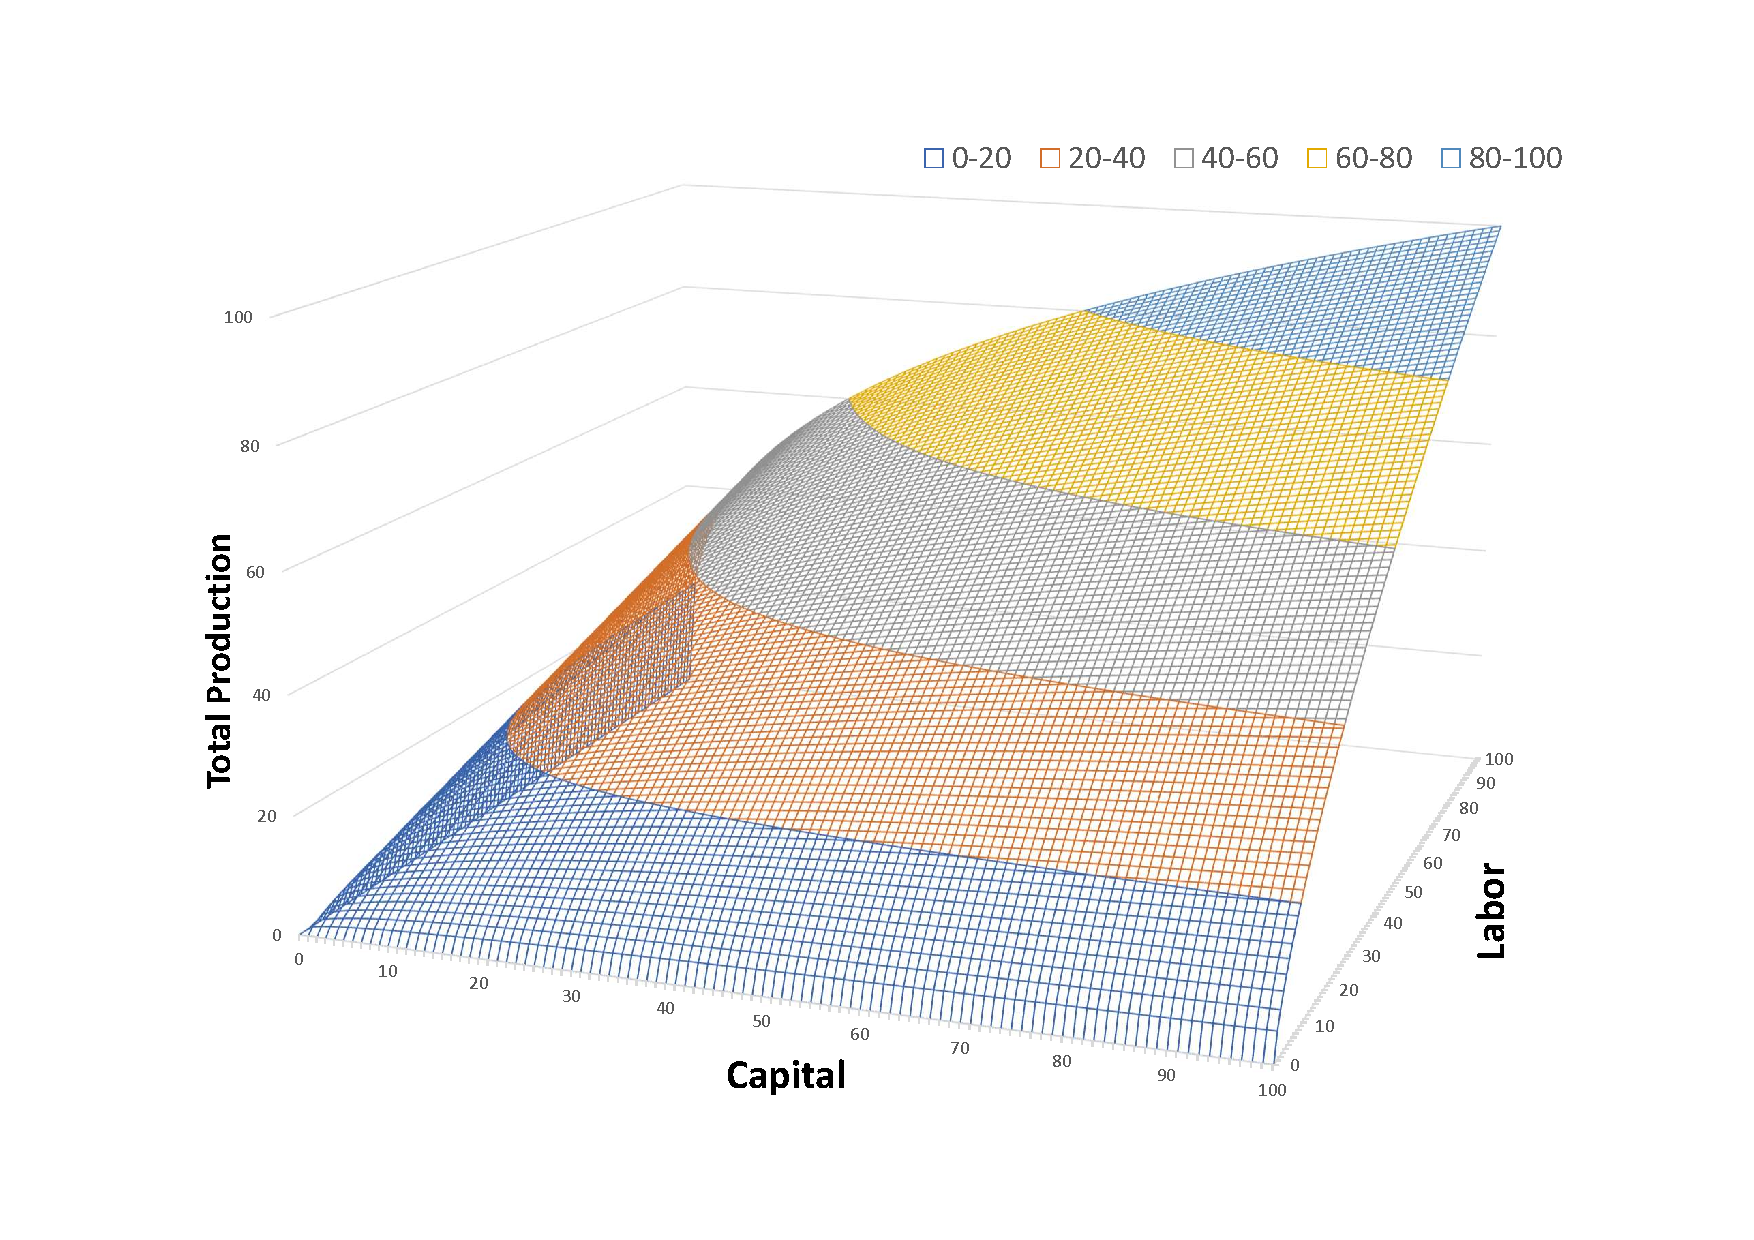
\includegraphics[width=\linewidth]{figs/cobb-douglas-crs.pdf}
      }
    }
\end{column}%
\hfill%
\begin{column}{.2\textwidth}
\begin{eqnarray*}
    Y &=& \bar{Z} K^{1/3} L^{2/3} \\
    \bar{Z} &=& 1
\end{eqnarray*}

Cobb-Douglas is Constant Returns to Scale in Capital and Labor jointly... but diminishing marginal returns while holding the other factor fixed...
\end{column}%
\end{columns}


\end{frame}

\begin{frame}{Profit Maximization}
  \begin{equation*}
    \max_{\{K,L\}} \pi  = \quad \underbrace{P \cdot F(K,L)}_{\text{revenues}} - \left( \underbrace{w \cdot L + r \cdot K}_{\text{costs}} \right)
  \end{equation*}

  \noindent where 
  \begin{wideitemize}
    \item $P$: price of the output good (if there is only one sector, we can normalize this $P=1$, num\'eraire)
    \item $F(K,L)$: production function
    \item $w$: wages
    \item $r$: rental rate on capital
  \end{wideitemize}
  
\end{frame}

\begin{frame}{Profit Maximization}
  \begin{equation*}
    \max_{\{K,L\}} \pi = \quad \underbrace{P \cdot F(K,L)}_{\text{revenues}} - \left( \underbrace{w \cdot L + r \cdot K}_{\text{costs}} \right)
  \end{equation*}

  First Order Conditions imply that, at the optimal:

  \begin{eqnarray*}
    \frac{\partial \pi}{\partial L} &=& 0 \implies P \cdot \frac{\partial F(K,L)}{\partial L} = P \cdot MPL = w \\
    \frac{\partial \pi}{\partial K} &=& 0 \implies P \cdot \frac{\partial F(K,L)}{\partial K} =  P \cdot MPK = r 
  \end{eqnarray*}

\end{frame}

\begin{frame}{Intuition for optimality result}
  
  \makebox[\linewidth][c]{
    \resizebox{0.8\linewidth}{!}{       
        \begin{tikzpicture}
        \pgfmathsetmacro{\alpha}{0.5}    % preference for computers
        \pgfmathsetmacro{\K}{1}    % labor endowment
        \pgfmathsetmacro{\A}{1}    % labor endowment
        
        \centering
        \begin{axis}[
            ylabel={$\textcolor{red}{P \times MPL}$, $w$ },
            xlabel={Used labor input: $L$},
            ymin=0, ymax=1.5,
            xmin=0, xmax=5,
            yticklabel=\empty,
            xticklabel=\empty,
            axis lines=left,
            enlargelimits=false,
            clip=false,
            axis on top,
            scaled x ticks=false,
            width=9cm, height=7cm,
            title style={font=\bfseries}
        ]
        
        % PPF: Q_C = (L/a_C) - (a_R/a_C) * Q_R
        \addplot[thick, red, domain=0:5] {(1-\alpha)*\A*\K^(\alpha)/x^(\alpha)};
        
        
        \addplot[dashed, purple, ->] coordinates {(0.5  , {(1-\alpha)*\A*\K^(\alpha)/0.5^(\alpha)}) (0.5 + 0.3, {(1-\alpha)*\A*\K^(\alpha)/0.5^(\alpha)} + 0.2)};
        \addplot[mark=*, only marks, purple, mark size=1pt] coordinates {(0.5, {(1-\alpha)*\A*\K^(\alpha)/0.5^(\alpha)})};
        \node[anchor=south west, purple] at (axis cs:0.5 + 0.3, {(1-\alpha)*\A*\K^(\alpha)/0.5^(\alpha)} + 0.25) {\scriptsize $P\times MPL > w^*$: hired too little};
        
        \pgfmathsetmacro{\Lb}{((1-\alpha)* \A / 0.5)^(1/\alpha) * \K}    % labor endowment
        
        \addplot[dashed, blue, ->] coordinates {(\Lb, {(1-\alpha)*\A*\K^(\alpha)/\Lb^(\alpha)}) (\Lb + 0.3, {(1-\alpha)*\A*\K^(\alpha)/\Lb^(\alpha)} + 0.2)};
        \addplot[mark=*, only marks, blue, mark size=1pt] coordinates {(\Lb, {(1-\alpha)*\A*\K^(\alpha)/\Lb^(\alpha)})};
        \node[anchor=south west, blue] at (axis cs:0.5 + 0.5, {(1-\alpha)*\A*\K^(\alpha)/\Lb^(\alpha)} + 0.2) {\scriptsize $P\times MPL = w^*$: hired just right};
        
        
        \addplot[dashed, black, ->] coordinates {(4  , {(1-\alpha)*\A*\K^(\alpha)/4^(\alpha)}) (4 + 0.3, {(1-\alpha)*\A*\K^(\alpha)/4^(\alpha)} + 0.1)};
        \addplot[mark=*, only marks, black, mark size=1pt] coordinates {(4, {(1-\alpha)*\A*\K^(\alpha)/4^(\alpha)})};
        \node[black] at (axis cs:4 + 0.3, {(1-\alpha)*\A*\K^(\alpha)/4^(\alpha)}+0.15) {\scriptsize $P\times MPL < w^*$: hired too much};
        
        
        \addplot[thick, dashed, domain=0:5] {0.5};
        
        \end{axis}
        
        \end{tikzpicture}
        
              }
    }

\end{frame}

\begin{frame}{Optimality Conditions for Demand with Cobb-Douglas}

  \begin{eqnarray*}
    Y &=& \bar{Z} (K^d)^{\beta} (L^d)^{1-\beta} \\
    P (1-\beta) \bar{Z} \left( \frac{K^d}{L^d} \right)^\beta  &=& w \\
    P \beta \bar{Z} \left( \frac{L^d}{K^d} \right)^{1-\beta}  &=& r 
  \end{eqnarray*}

\end{frame}

\begin{frame}{Optimality Conditions for Demand with Cobb-Douglas}

  Note that we can derive a labor demand and capital demand schedule from each of those, which are decreasing in factor prices:

  \begin{eqnarray*}
    L^d &=& \left( \frac{(1-\beta) \cdot A \cdot P}{w} \right)^{\frac{1}{\beta}} \cdot K^d \\
    K^d &=& \left( \frac{\beta \cdot A \cdot P}{r} \right)^{\frac{1}{1-\beta}} \cdot L^d
  \end{eqnarray*}

\end{frame}

\begin{frame}{Demand}
\begin{figure}[htbp!]

\begin{subfigure}{}
\resizebox{0.48\textwidth}{!}{%
        \begin{tikzpicture}
        \pgfmathsetmacro{\alpha}{2/3}
        \pgfmathsetmacro{\K}{1}
        \pgfmathsetmacro{\A}{1}
        
        \begin{axis}[
            ylabel={$\textcolor{red}{L^d(w)}$, $w$ },
            xlabel={Used labor input: $L$},
            ymin=0, ymax=1.5,
            xmin=0, xmax=5,
            yticklabel=\empty,
            xticklabel=\empty,
            axis lines=left,
            enlargelimits=false,
            clip=false,
            axis on top,
            scaled x ticks=false,
            width=9cm, height=7cm,
            title={Labor demand curve}
        ]
        \addplot[thick, red, domain=0:5] {(1-\alpha)*\A*\K^(\alpha)/x^(\alpha)};
        \addplot[thick, dashed, domain=0:5] {0.5};
        %\addplot[dashed, gray] coordinates {({((1-\alpha)*\A/0.5)^(1/\alpha)*\K}, 0.5) ({((1-\alpha)*\A/0.5)^(1/\alpha)*\K},0)};

        %\node at (axis cs:3.5,0.03) {\Large $\mathcal{Y}_{US}$};
        \node at (axis cs:-0.125,0.5) {\scriptsize $w^*$};
        
        \end{axis}
        \end{tikzpicture}
}
\end{subfigure}
%
\begin{subfigure}{}
\resizebox{0.48\textwidth}{!}{%

        \begin{tikzpicture}
        \pgfmathsetmacro{\alpha}{1/3}
        \pgfmathsetmacro{\K}{1}
        \pgfmathsetmacro{\A}{1}
        
        \begin{axis}[
            ylabel={$\textcolor{blue}{K^d(r)}$, $r$ },
            xlabel={Used capital input: $K$},
            ymin=0, ymax=1.5,
            xmin=0, xmax=5,
            yticklabel=\empty,
            xticklabel=\empty,
            axis lines=left,
            enlargelimits=false,
            clip=false,
            axis on top,
            scaled x ticks=false,
            width=9cm, height=7cm,
            title={Capital demand curve}
        ]
        \addplot[thick, blue, domain=0:5] {(1-\alpha)*\A*\K^(\alpha)/x^(\alpha)};
        \addplot[thick, dashed, domain=0:5] {0.5};

        %\node at (axis cs:3.5,0.03) {\Large $\mathcal{Y}_{US}$};
        \node at (axis cs:-0.125,0.5) {\scriptsize $r^*$};
        %\node at (axis cs:({((1-\alpha)*\A/0.5)^(1/\alpha)*\K},-0.1) {\scriptsize $\bar{K}$};
        \end{axis}
        \end{tikzpicture}
}

\end{subfigure}

\end{figure}

\end{frame}

\begin{frame}{Supply side of the economy is simple}

\begin{wideitemize}
    \item Households supply labor and capital inelastically.
    \item Prices adjust to ensure that supply equals demand (market clearing condition) 
\end{wideitemize}


  \begin{eqnarray*}
     L^d &=& L^s = \bar{L} \qquad \text{(parameter)} \\
     K^d &=& K^s = \bar{K} \qquad \text{(parameter)}
  \end{eqnarray*}

\end{frame}



\begin{frame}{Supply}
\begin{figure}[htbp!]

\begin{subfigure}{}
\resizebox{0.48\textwidth}{!}{%
        \begin{tikzpicture}
        \pgfmathsetmacro{\alpha}{2/3}
        \pgfmathsetmacro{\K}{1}
        \pgfmathsetmacro{\A}{1}
        
        \begin{axis}[
            ylabel={$\textcolor{red}{L^s}$, $w$ },
            xlabel={Used labor input: $L$},
            ymin=0, ymax=1.5,
            xmin=0, xmax=5,
            yticklabel=\empty,
            xticklabel=\empty,
            axis lines=left,
            enlargelimits=false,
            clip=false,
            axis on top,
            scaled x ticks=false,
            width=9cm, height=7cm,
            title={Labor supply curve}
        ]
        %\addplot[thick, red, domain=0:5] {(1-\alpha)*\A*\K^(\alpha)/x^(\alpha)};
        \addplot[thick, dashed, domain=0:5] {0.5};
        \addplot[thick, red] coordinates {({((1-\alpha)*\A/0.5)^(1/\alpha)*\K}, 1.5) ({((1-\alpha)*\A/0.5)^(1/\alpha)*\K},0)};

        %\node at (axis cs:3.5,0.03) {\Large $\mathcal{Y}_{US}$};
        \node at (axis cs:-0.125,0.5) {\scriptsize $w^*$};
        \node at (axis cs:({((1-\alpha)*\A/0.5)^(1/\alpha)*\K},-0.1) {\scriptsize $\bar{L}$};
        
        \end{axis}
        \end{tikzpicture}
}
\end{subfigure}
%
\begin{subfigure}{}
\resizebox{0.48\textwidth}{!}{%

        \begin{tikzpicture}
        \pgfmathsetmacro{\alpha}{1/3}
        \pgfmathsetmacro{\K}{1}
        \pgfmathsetmacro{\A}{1}
        
        \begin{axis}[
            ylabel={$\textcolor{blue}{K^s}$, $r$ },
            xlabel={Used labor input: $K$},
            ymin=0, ymax=1.5,
            xmin=0, xmax=5,
            yticklabel=\empty,
            xticklabel=\empty,
            axis lines=left,
            enlargelimits=false,
            clip=false,
            axis on top,
            scaled x ticks=false,
            width=9cm, height=7cm,
            title={Capital supply curve}
        ]
        %\addplot[thick, blue, domain=0:5] {(1-\alpha)*\A*\K^(\alpha)/x^(\alpha)};
        \addplot[thick, dashed, domain=0:5] {0.5};
        \addplot[thick, blue] coordinates {({((1-\alpha)*\A/0.5)^(1/\alpha)*\K}, 1.5) ({((1-\alpha)*\A/0.5)^(1/\alpha)*\K},0)};

        %\node at (axis cs:3.5,0.03) {\Large $\mathcal{Y}_{US}$};
        \node at (axis cs:-0.125,0.5) {\scriptsize $r^*$};
        \node at (axis cs:({((1-\alpha)*\A/0.5)^(1/\alpha)*\K},-0.1) {\scriptsize $\bar{K}$};
        \end{axis}
        \end{tikzpicture}
}

\end{subfigure}

\end{figure}
\end{frame}


\begin{frame}{General Equilibrium}

\Large{Endogeneous Variables: $Y, K, L, w, r$, \quad Num\'eraire: $P=1$}

\vspace{20pt}

\normalsize Five equations for five unknowns

  \begin{eqnarray}
    Y &=& \bar{Z} (K)^{\alpha} (L)^{1-\alpha} \\
    P (1-\alpha) \bar{Z} \left( \frac{K}{L} \right)^\alpha  &=& w \\
    P \alpha \bar{Z} \left( \frac{L}{K} \right)^{1-\alpha}  &=& r  \\
     L &=& \bar{L} = L^s  \\
     K &=& \bar{K} = K^s
  \end{eqnarray}

\end{frame}

\begin{frame}{Solution to the Production Model}

Replacing the market clearing condition in and normalizing $P=1$ to be the num\'eraire of this economy:

  \begin{eqnarray}
    Y^* &=& \bar{Z} (\bar{K})^{\alpha} (\bar{L})^{1-\alpha} \\
    w^* &=& (1-\alpha) \bar{Z} \left( \frac{\bar{K}}{\bar{L}} \right)^\alpha  \\
     r^* &=&  \alpha \bar{Z} \left( \frac{\bar{L}}{\bar{K}} \right)^{1-\alpha}  \\
     L^* &=& \bar{L}  \\
     K^* &=& \bar{K}
  \end{eqnarray}

Note that everything on the right-hand side of the equations is a parameter, so this is indeed an explicit solution!
\end{frame}

\begin{frame}{Numerical Example}

Suppose $\bar{K} = 20, \bar{L} = 160, \bar{Z}=1, \alpha=\frac{1}{3}$. What is the solution to the Production Model? Replacing in the set of equations before:

  \begin{eqnarray*}
    Y^* &=&  (20)^{\frac{1}{3}}  (160)^{\frac{2}{3}} = 80 \\
    w^* &=& \frac{2}{3} \left( \frac{20}{160} \right)^{\frac{1}{3}} = \frac{1}{3} \\
     r^* &=&  \frac{1}{3} \left( \frac{160}{20} \right)^{\frac{2}{3}} = \frac{4}{3}  \\
     L^* &=& 160  \\
     K^* &=& 20
  \end{eqnarray*}
\end{frame}


\begin{frame}{Solution to the Model in General Equilibrium}
\begin{figure}[htbp!]

\begin{subfigure}{}
\resizebox{0.48\textwidth}{!}{%
        \begin{tikzpicture}
        \pgfmathsetmacro{\alpha}{2/3}
        \pgfmathsetmacro{\K}{1}
        \pgfmathsetmacro{\A}{1}
        
        \begin{axis}[
            ylabel={$\textcolor{red}{L^d(w)}$, $w$ },
            xlabel={Used labor input: $L$},
            ymin=0, ymax=1.5,
            xmin=0, xmax=5,
            yticklabel=\empty,
            xticklabel=\empty,
            axis lines=left,
            enlargelimits=false,
            clip=false,
            axis on top,
            scaled x ticks=false,
            width=9cm, height=7cm,
            title={Labor supply curve}
        ]
        \addplot[thick, red, domain=0:5] {(1-\alpha)*\A*\K^(\alpha)/x^(\alpha)};
        \addplot[thick, dashed, domain=0:5] {0.5};
        \addplot[thick, red] coordinates {({((1-\alpha)*\A/0.5)^(1/\alpha)*\K}, 1.5) ({((1-\alpha)*\A/0.5)^(1/\alpha)*\K},0)};

        %\node at (axis cs:3.5,0.03) {\Large $\mathcal{Y}_{US}$};
        \node at (axis cs:-0.125,0.5) {\scriptsize $w^*$};
        \node at (axis cs:({((1-\alpha)*\A/0.5)^(1/\alpha)*\K},-0.1) {\scriptsize $\bar{L}$};
        
        \end{axis}
        \end{tikzpicture}
}
\end{subfigure}
%
\begin{subfigure}{}
\resizebox{0.48\textwidth}{!}{%

        \begin{tikzpicture}
        \pgfmathsetmacro{\alpha}{1/3}
        \pgfmathsetmacro{\K}{1}
        \pgfmathsetmacro{\A}{1}
        
        \begin{axis}[
            ylabel={$\textcolor{blue}{K^d(r)}$, $r$ },
            xlabel={Used labor input: $L$},
            ymin=0, ymax=1.5,
            xmin=0, xmax=5,
            yticklabel=\empty,
            xticklabel=\empty,
            axis lines=left,
            enlargelimits=false,
            clip=false,
            axis on top,
            scaled x ticks=false,
            width=9cm, height=7cm,
            title={Capital supply curve}
        ]
        \addplot[thick, blue, domain=0:5] {(1-\alpha)*\A*\K^(\alpha)/x^(\alpha)};
        \addplot[thick, dashed, domain=0:5] {0.5};
        \addplot[thick, blue] coordinates {({((1-\alpha)*\A/0.5)^(1/\alpha)*\K}, 1.5) ({((1-\alpha)*\A/0.5)^(1/\alpha)*\K},0)};

        %\node at (axis cs:3.5,0.03) {\Large $\mathcal{Y}_{US}$};
        \node at (axis cs:-0.125,0.5) {\scriptsize $r^*$};
        \node at (axis cs:({((1-\alpha)*\A/0.5)^(1/\alpha)*\K},-0.1) {\scriptsize $\bar{K}$};
        \end{axis}
        \end{tikzpicture}
}

\end{subfigure}

\end{figure}
\end{frame}


\begin{frame}{Numerical Example}

Now suppose the total available capital changes to $\bar{K}' = 10$. What happens?

  \begin{eqnarray*}
    Y^{**} &=&  (10)^{\frac{1}{3}}  (160)^{\frac{2}{3}} = 63.5 \\
    w^{**} &=& \frac{2}{3} \left( \frac{10}{160} \right)^{\frac{1}{3}} = 0.26 \\
     r^{**} &=&  \frac{1}{3} \left( \frac{160}{10} \right)^{\frac{2}{3}} = 2.11  \\
     L^{**} &=& 160  \\
     K^{**} &=& 10
  \end{eqnarray*}
\end{frame}

\begin{frame}{Numerical Example: Graphical Representation of Comparative Statics}

  \makebox[\linewidth][c]{
    \resizebox{\linewidth}{!}{
    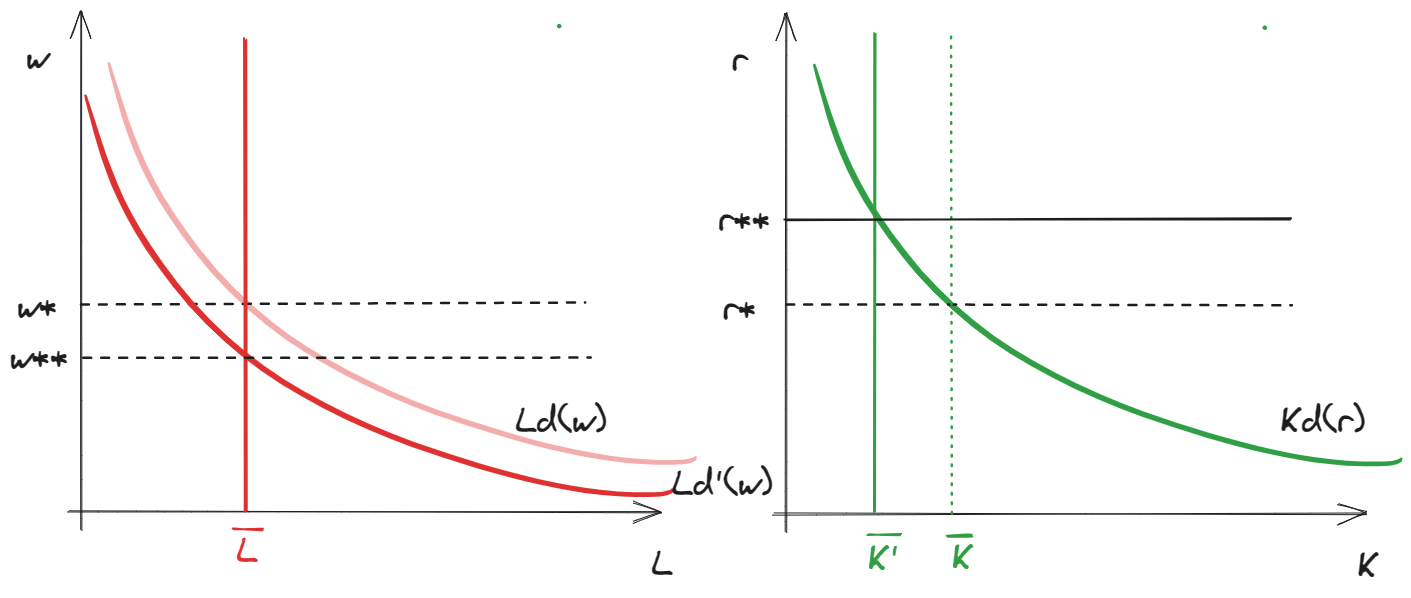
\includegraphics{figs/productioncomparativestat.png}
      }
    }

\end{frame}


\end{document}
